

%% AAPT Physics Olympiad F=ma Questions
%%----------------------------------------


%% this section contains 20 problems


%% PhysicsOlympiad 2015
%%----------------------------------------
\element{aapt}{ %% Olympiad-A8
\begin{question}{Olympiad-2015-q12}
    %%The following information applies to questions 12 and 13
    A pendulum consists of a small bob of mass $m$ attached to a fixed point by a string of length $L$.
    The pendulum bob swings down from rest from an initial angle $\theta_{max} < \ang{90}$.
    %% Begin Question
    Which of the following statements about the pendulum bob's acceleration is true?
    \begin{choices}
        \wrongchoice{The magnitude of the acceleration is constant for the motion.}
        \wrongchoice{The magnitude of the acceleration at the lowest point is $g$, the acceleration of free fall.}
        \wrongchoice{The magnitude of the acceleration is zero at some point of the pendulum’s swing.}
        \wrongchoice{The acceleration is always directed toward the center of the circle.}
      \correctchoice{The acceleration at the bottom of the swing is pointing vertically upward.}
    \end{choices}
\end{question}
}

\element{aapt}{ %% Olympiad-A8
\begin{question}{Olympiad-2015-q13}
    %%The following information applies to questions 12 and 13
    A pendulum consists of a small bob of mass $m$ attached to a fixed point by a string of length $L$.
    The pendulum bob swings down from rest from an initial angle $\theta_{max}<\ang{90}$.
    %% Begin Question
    Consider the pendulum bob when it is at an angle $\theta=\dfrac{1}{2}\theta_{max}$ on the way up (moving toward $\theta_{max}$).
    What is the direction of the acceleration vector?
    \begin{multicols}{2}
    \begin{choices}
        \AMCboxDimensions{down=-1.5cm}
        \wrongchoice{
            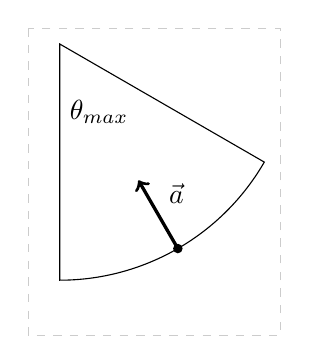
\begin{tikzpicture}
                \draw[dashed,white!80!black] (-0.4,0.2) rectangle (2.8,-3.7);
                \draw (0,0) -- (0,-3) arc (270:330:3) -- cycle;
                \draw[fill] (300:3) circle (1.5pt);
                \node[anchor=center] at (300:1) {$\theta_{max}$};
                \draw[very thick,->] (300:3)  -- ++(120:1) node[pos=0.5,anchor=south west] {$\vec{a}$};
            \end{tikzpicture}
        }
        \wrongchoice{
            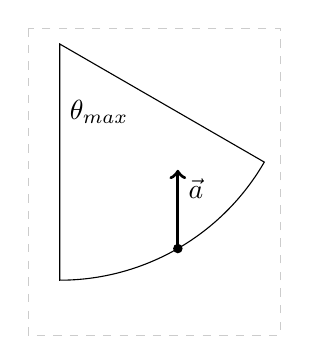
\begin{tikzpicture}
                \draw[dashed,white!80!black] (-0.4,0.2) rectangle (2.8,-3.7);
                \draw (0,0) -- (0,-3) arc (270:330:3) -- cycle;
                \draw[fill] (300:3) circle (1.5pt);
                \node[anchor=center] at (300:1) {$\theta_{max}$};
                \draw[very thick,->] (300:3)  -- ++(90:1) node[pos=0.5,anchor=south west] {$\vec{a}$};
            \end{tikzpicture}
        }
        \wrongchoice{
            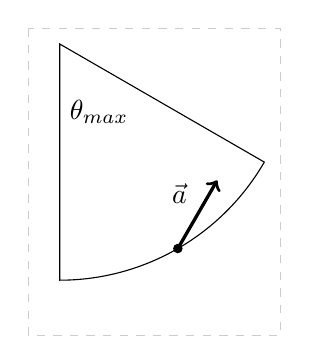
\begin{tikzpicture}
                \draw[dashed,white!80!black] (-0.4,0.2) rectangle (2.8,-3.7);
                \draw (0,0) -- (0,-3) arc (270:330:3) -- cycle;
                \draw[fill] (300:3) circle (1.5pt);
                \node[anchor=center] at (300:1) {$\theta_{max}$};
                \draw[very thick,->] (300:3)  -- ++(60:1) node[pos=0.5,anchor=south east] {$\vec{a}$};
            \end{tikzpicture}
        }
        %% ANS is D: angle is 135 if \theta=60, \theta/2=30
        %% changed to 160 to avoid confusion with A
        \correctchoice{
            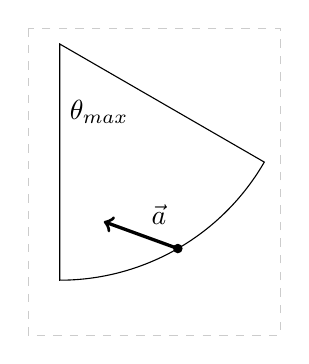
\begin{tikzpicture}
                \draw[dashed,white!80!black] (-0.4,0.2) rectangle (2.8,-3.7);
                \draw (0,0) -- (0,-3) arc (270:330:3) -- cycle;
                \draw[fill] (300:3) circle (1.5pt);
                \node[anchor=center] at (300:1) {$\theta_{max}$};
                \draw[very thick,->] (300:3)  -- ++(160:1) node[pos=0.5,anchor=south west] {$\vec{a}$};
            \end{tikzpicture}
        }
        \wrongchoice{
            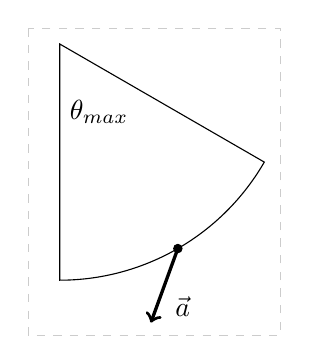
\begin{tikzpicture}
                \draw[dashed,white!80!black] (-0.4,0.2) rectangle (2.8,-3.7);
                \draw (0,0) -- (0,-3) arc (270:330:3) -- cycle;
                \draw[fill] (300:3) circle (1.5pt);
                \node[anchor=center] at (300:1) {$\theta_{max}$};
                \draw[very thick,->] (300:3)  -- ++(250:1) node[pos=0.5,anchor=north west] {$\vec{a}$};
            \end{tikzpicture}
        }
    \end{choices}
    \end{multicols}
\end{question}
}

\element{aapt}{ %% Olympiad-A8
\begin{question}{Olympiad-2015-q24}
    The speed of a transverse wave on a long cylindrical steel string is given by
    \begin{equation*}
        v = \sqrt{\dfrac{TL}{M}}\, ,
    \end{equation*}
    where $T$ is the tension in the string,
        $M$ is the mass, and $L$ is the length of the string.
    Ignore any string stiffness,
        and assume that it does not stretch when tightened.
    Consider two steel strings of the same length,
        the first with radius $r_1$ and a second thicker string with radius $r_2=4r_1$.
    Each string is tightened to the maximum possible tension without breaking.
    What is the ratio $\dfrac{f_1}{f_2}$ of the fundamental frequencies of vibration on the two strings?
    \begin{multicols}{3}
    \begin{choices}
      \correctchoice{$1$}
        \wrongchoice{$\sqrt{2}$}
        \wrongchoice{$2$}
        \wrongchoice{$2\sqrt{2}$}
        \wrongchoice{$4$}
    \end{choices}
    \end{multicols}
\end{question}
}

\element{aapt}{ %% Olympiad-A8
\begin{question}{Olympiad-2015-q25}
    Two identical carts $A$ and $B$ each with mass $m$ are connected via a spring with spring constant $k$.
    Two additional springs, identical to the first,
        connect the carts to two fixed points.
    The carts are free to oscillate under the effect of the springs in one dimensional frictionless motion.
    \begin{center}
    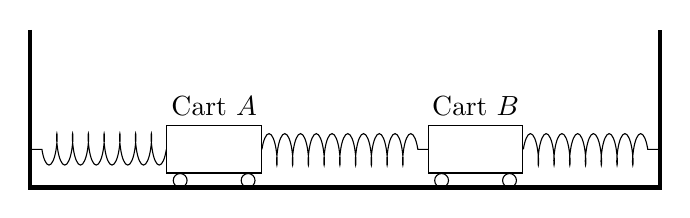
\begin{tikzpicture}
        \draw[ultra thick] (-4,2) -- (-4,0) -- (4,0) -- (4,2);
        %% Carts
        \node[draw,anchor=south,minimum width=1.2cm,minimum height=0.6cm] (A) at (-1.66,0.5em) {};
        \node[draw,anchor=south,minimum width=1.2cm,minimum height=0.6cm] (B) at (+1.66,0.5em) {};
        \node[anchor=south] at (A.north) {Cart $A$};
        \node[anchor=south] at (B.north) {Cart $B$};
        %% Wheels
        \draw (A.south west) ++(+0.5em,-0.25em) circle (0.25em);
        \draw (A.south east) ++(-0.5em,-0.25em) circle (0.25em);
        \draw (B.south west) ++(+0.5em,-0.25em) circle (0.25em);
        \draw (B.south east) ++(-0.5em,-0.25em) circle (0.25em);
        %% Spring
        \draw[decoration={aspect=0.2,segment length=2mm,amplitude=2mm,coil},decorate] (A.west) -- ++(180:1.75);
        \draw[decoration={aspect=0.2,segment length=2mm,amplitude=2mm,coil},decorate] (A.east) -- (B.west);
        \draw[decoration={aspect=0.2,segment length=2mm,amplitude=2mm,coil},decorate] (B.east) -- ++(0:1.75);
    \end{tikzpicture}
    \end{center}
    Under suitable initial conditions,
        the two carts will oscillate in phase according to
    \begin{equation*}
        x_A (t) = x_0 \sin\omega_1 t = x_B (t)
    \end{equation*}
    where $x_A$ and $x_B$ are the locations of carts $A$ and $B$ relative to their respective equilibrium positions.
    Under other suitable initial conditions,
        the two carts will oscillate exactly out of phase according to
    \begin{equation*}
        x_A (t) = x_0 \sin\omega_2 t = -x_B(t)
    \end{equation*}
    Determine the ratio $\dfrac{\omega_2}{\omega_1}$:
    \begin{multicols}{3}
    \begin{choices}
      \correctchoice{$\sqrt{3}$}
        \wrongchoice{$2$}
        \wrongchoice{$2\sqrt{2}$}
        \wrongchoice{$3$}
        \wrongchoice{$5$}
    \end{choices}
    \end{multicols}
\end{question}
}


%% PhysicsOlympiad 2014
%%----------------------------------------
\element{aapt}{ %% Olympiad-A8
\begin{question}{Olympiad-2014-q08}
    An object of mass $M$ is hung on a vertical spring of spring constant $k$
        and is set into vertical oscillations.
    The period of this oscillation is $T_0$.
    The spring is then cut in half and the same mass is attached and the system
        is set up to oscillate on a frictionless inclined plane making an angle $\theta$
        to the horizontal.
    Determine the period of the oscillations on the inclined plane in terms of $T_0$.
    \begin{multicols}{3}
    \begin{choices}
        \wrongchoice{$T_0$}
        \wrongchoice{$\dfrac{T_0}{2}$}
        \wrongchoice{$2T_0\sin\theta$}
      \correctchoice{$\dfrac{T_0}{\sqrt{2}}$}
        \wrongchoice{$\dfrac{T_0\sin\theta}{\sqrt{2}}$}
    \end{choices}
    \end{multicols}
\end{question}
}

\newcommand{\OlympiadTwentyFourteenQTwelve}{
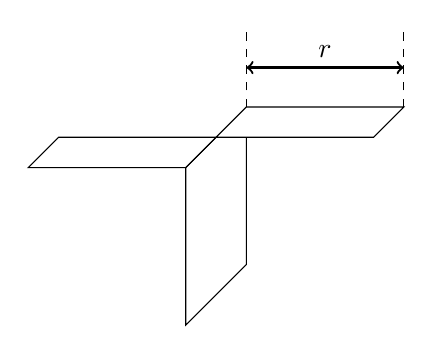
\begin{tikzpicture}
    %% Left wing
    \draw (0,0,0) -- (-2,0,0) -- (-2,0,-1) -- (0,0,-1) -- cycle;
    %% Main body
    \draw (0,0,0) -- (0,-2,0) -- (0,-2,-2) -- (0,0,-2) -- cycle;
    %% Right wing
    \draw[fill=white] (0,0,-1) -- (0,0,-2) -- (2,0,-2) -- (2,0,-1) -- cycle;
    \draw[dashed] (0,0,-2) -- (0,1,-2);
    \draw[dashed] (2,0,-2) -- (2,1,-2);
    \draw[thick,<->] (0,0.5,-2) -- (2,0.5,-2) node[pos=0.5,anchor=south] {$r$};
\end{tikzpicture}
}


%% PhysicsOlympiad 2013
%%----------------------------------------
\element{aapt}{ %% Olympiad-A8
\begin{question}{Olympiad-2013-q19}
    %The following information applies to questions 19, 20, and 21.
    A simple pendulum experiment is constructed from a point mass $m$ attached to a pivot by a massless rod of length $L$ in a constant gravitational field.
    The rod is released from an angle $\theta_0 < \pi/2$ at rest and the period of motion is found to be $T_0$.
    Ignore air resistance and friction.
    %% Start question
    At what angle $\theta_g$ during the swing is the tension in the rod the greatest?
    \begin{choices}
        \wrongchoice{The tension is the greatest at the point $θ_g=\theta_0$.}
      \correctchoice{The tension is the greatest at the point $θ_g=0$.}
        \wrongchoice{The tension is the greatest at an angle $θ_g$ with $\theta < θ_g < θ_0$.}
        \wrongchoice{The tension is constant.}
        \wrongchoice{None of the provided are true for all values of $θ_0$ with $0 < θ_0 < \frac{\pi}{2}$.}
    \end{choices}
\end{question}
}

\element{aapt}{ %% Olympiad-A8
\begin{question}{Olympiad-2013-q20}
    %The following information applies to questions 19, 20, and 21.
    A simple pendulum experiment is constructed from a point mass $m$ attached to a pivot by a massless rod of length $L$ in a constant gravitational field.
    The rod is released from an angle $\theta_0 < \pi/2$ at rest and the period of motion is found to be $T_0$.
    Ignore air resistance and friction.
    %% Start question
    What is the maximum value of the tension in the rod?
    \begin{multicols}{2}
    \begin{choices}
        \wrongchoice{$mg$}
        \wrongchoice{$2mg$}
        \wrongchoice{$\dfrac{mL\theta_0}{T_0^2}$}
        \wrongchoice{$mg \sin\theta_0$}
      \correctchoice{$mg\left( 3 - 2\cos\theta_0 \right)$}
    \end{choices}
    \end{multicols}
\end{question}
}

\element{aapt}{ %% Olympiad-A8
\begin{question}{Olympiad-2013-q21}
    %The following information applies to questions 19, 20, and 21.
    A simple pendulum experiment is constructed from a point mass $m$ attached to a pivot by a massless rod of length $L$ in a constant gravitational field.
    The rod is released from an angle $\theta_0 < \pi/2$ at rest and the period of motion is found to be $T_0$.
    Ignore air resistance and friction.
    %% Start question
    The experiment is repeated with a new pendulum with a rod of length $4L$,
        using the same angle $\theta_0$, and the period of motion is found to be $T$.
    Which of the following statements is correct?
    \begin{choices}
      \correctchoice{$T = 2T_0$ regardless of the value of $\theta_0$.}
        \wrongchoice{$T > 2T_0$ with $T\approx{}2T_0$ if $\theta_0 \ll 1$.}
        \wrongchoice{$T < 2T_0$ with $T\approx{}2T_0$ if $\theta_0 \ll 1$.}
        \wrongchoice{$T > 2T_0$ for some values of $\theta_0$ and $T<2T_0$ for other values of $\theta_0$.}
        \wrongchoice{$T_0$ and $T$ are undefined because the motion is not periodic unless $\theta_0 \ll 1$.}
    \end{choices}
\end{question}
}


%% PhysicsOlympiad 2012
%%----------------------------------------
\element{aapt}{ %% Olympiad-A8
\begin{question}{Olympiad-2012-q16}
    Inside a cart that is accelerating horizontally at acceleration $\vec{a}$,
        there is a block of mass $M$ connected to two light springs of
        force constants $k_1$ and $k_2$.
    \begin{center}
    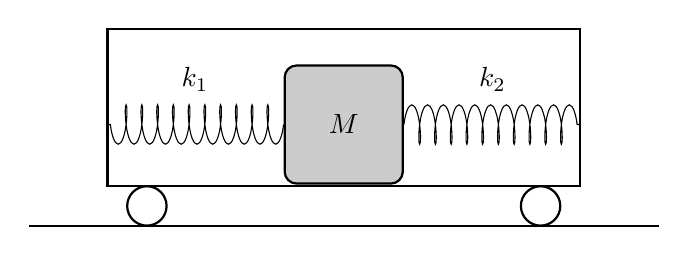
\begin{tikzpicture}
        %% Floor
        \draw[thick] (-4,0) -- (4,0);
        %% Cart
        \draw[thick] (-3,0.5) rectangle (3,2.5);
        %% Wheels
        \draw[thick] (-2.5,0.25) circle (0.25);
        \draw[thick] (+2.5,0.25) circle (0.25);
        %% Mass
        \node[thick,draw,minimum size=1.5cm,fill=white!80!black,rounded corners=1ex,anchor=south] (M) at (0,0.52) {$M$};
        %% spring
        \draw[decoration={aspect=0.2,segment length=2.0mm,amplitude=2.5mm,coil},decorate] (M.west) -- ++(180:2.25) node[pos=0.5,anchor=south,yshift=3mm] {$k_1$};
        \draw[decoration={aspect=0.2,segment length=2.0mm,amplitude=2.5mm,coil},decorate] (M.east) -- ++(0:2.25) node[pos=0.5,anchor=south,yshift=3mm] {$k_2$};
    \end{tikzpicture}
    \end{center}
    The block can move without friction horizontally.
    Find the vibration frequency of the block.
    \begin{choices}
        \wrongchoice{$\dfrac{1}{2\pi}\sqrt{\dfrac{k_1+k_2}{M} + a}$}
        \wrongchoice{$\dfrac{1}{2\pi}\sqrt{\dfrac{k_1 k_2}{\left(k_1+k_2\right)M}}$}
        \wrongchoice{$\dfrac{1}{2\pi}\sqrt{\dfrac{k_1 k_2}{\left(k_1+k_2\right)M} + a}$}
        \wrongchoice{$\dfrac{1}{2\pi}\sqrt{\dfrac{|k_1-k_2|}{M}}$}
      \correctchoice{$\dfrac{1}{2\pi}\sqrt{\dfrac{k_1+k_2}{M}}$}
    \end{choices}
\end{question}
}

\element{aapt}{ %% Olympiad-A8
\begin{question}{Olympiad-2012-q17}
    Shown below is a log/log plot for the data collected of amplitude
        and period of oscillation for certain non-linear oscillator.
    \begin{center}
    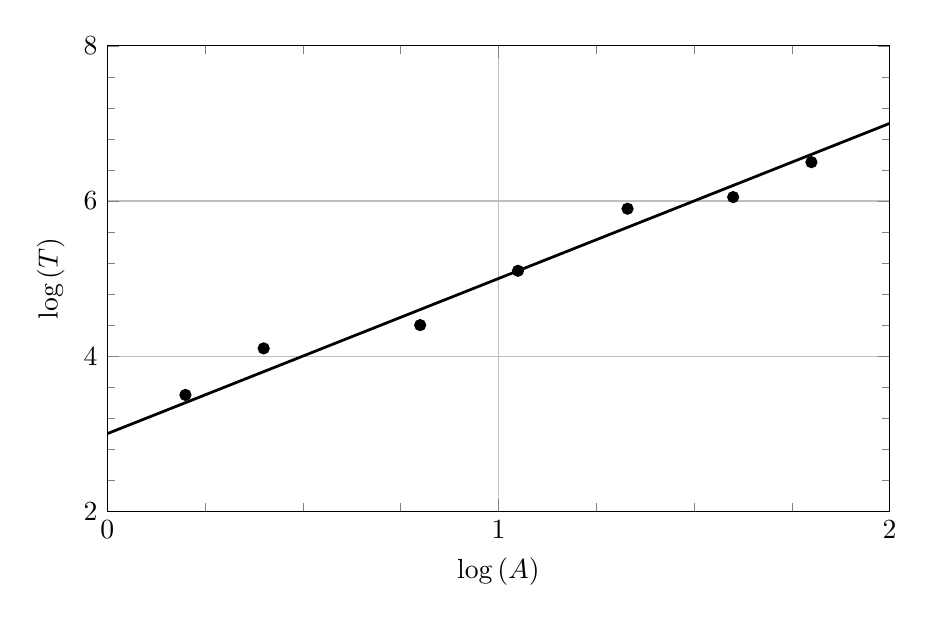
\begin{tikzpicture}
        \begin{axis}[
            xlabel={$\log\left(A\right)$},
            xtick={0,1,2},
            minor x tick num=3,
            ylabel={$\log\left(T\right)$},
            ytick={2,4,6,8},
            minor y tick num=4,
            grid=major,
            xmin=0,xmax=2,
            ymin=2,ymax=8,
            width=0.95\columnwidth,
            height=0.618\columnwidth,
        ]
        \addplot[line width=1pt,domain=0:2]{3 + 2*x};
        \addplot[mark=*,only marks] plot coordinates { (0.20,3.5) (0.4,4.1) (0.80,4.4) (1.05,5.1) (1.33,5.9) (1.6,6.05) (1.8,6.5) };
        \end{axis}
    \end{tikzpicture}
    \end{center}
    According to the data,
        the relationship between period $T$ and amplitude $A$ is best given by
    \begin{choices}
      \correctchoice{$T=\num{1000}A^2$}
        \wrongchoice{$T=\num{1000}A^3$}
        \wrongchoice{$T=2A+3$}
        \wrongchoice{$T=3\sqrt{A}$}
        \wrongchoice{Period is independent of amplitude for oscillating systems}
    \end{choices}
\end{question}
}

\element{aapt}{ %% Olympiad-A8
\begin{question}{Olympiad-2012-q18}
    A mass hangs from the ceiling of a box by an ideal spring.
    With the box held fixed,
        the mass is given an initial velocity and oscillates with purely vertical motion.
    When the mass reaches the lowest point of its motion,
        the box is released and allowed to fall.
    To an observer inside the box,
        which of the following quantities does not change when the box is released?
    Ignore air resistance.
    \begin{choices}
        \wrongchoice{The amplitude of the oscillation}
      \correctchoice{The period of the oscillation}
        \wrongchoice{The maximum speed reached by the mass}
        \wrongchoice{The height at which the mass reaches its maximum speed}
        \wrongchoice{The maximum height reached by the mass}
    \end{choices}
\end{question}
}


%% PhysicsOlympiad 2011
%%----------------------------------------
\element{aapt}{ %% Olympiad-A8
\begin{question}{Olympiad-2011-q10}
    Which of the following changes will result in an \emph{increase}
        in the period of a simple pendulum?
    \begin{choices}
        \wrongchoice{Decrease the length of the pendulum}
        \wrongchoice{Increase the mass of the pendulum}
      \correctchoice{Increase the amplitude of the pendulum swing}
        \wrongchoice{Operate the pendulum in an elevator that is accelerating upward}
        \wrongchoice{Operate the pendulum in an elevator that is moving downward at constant speed.}
    \end{choices}
\end{question}
}

\element{aapt}{ %% Olympiad-A7
\begin{question}{Olympiad-2011-q19}
    A particle of mass \SI{2.00}{\kilo\gram} moves under a force given by
    \begin{equation*}
        \mathbf{F} = -\left(\SI{8.00}{\newton\per\meter}\right)
            \left( x\hat{i} + y\hat{j}\right)
    \end{equation*}
    where $\hat{i}$ and $\hat{j}$ are unit vectors in the
        $x$ and $y$ directions.
    the particle is placed at the origin with an initial velocity
    \begin{equation*}
        \mathbf{v} = \left(\SI{3.00}{\meter\per\second}\right)\hat{i}
            + \left(\SI{4.00}{\meter\per\second}\right)\hat{j} .
    \end{equation*}
    After how much time will the particle first return to the origin?
    \begin{multicols}{3}
    \begin{choices}
        \wrongchoice{\SI{0.785}{\second}}
        \wrongchoice{\SI{1.29}{\second}}
      \correctchoice{\SI{1.57}{\second}}
        \wrongchoice{\SI{2.00}{\second}}
        \wrongchoice{\SI{3.14}{\second}}
    \end{choices}
    \end{multicols}
\end{question}
}

\element{aapt}{ %% Olympiad-A3
\begin{question}{Olympiad-2011-q20}
    A particle of mass \SI{2.00}{\kilo\gram} moves under a force given by
    \begin{displaymath}
        \mathbf{F} = -\left(\SI{8.00}{\newton\per\meter}\right)
            \left( x\hat{i} + y\hat{j}\right)
    \end{displaymath}
    where $\hat{i}$ and $\hat{j}$ are unit vectors in the
        $x$ and $y$ directions.
    the particle is placed at the origin with an initial velocity
    \begin{equation*}
        \mathbf{v} = \left(\SI{3.00}{\meter\per\second}\right)\hat{i}
            + \left(\SI{4.00}{\meter\per\second}\right)\hat{j} .
    \end{equation*}
    What is the maximum distance between the particle and the origin?
    \begin{multicols}{3}
    \begin{choices}
        \wrongchoice{\SI{2.00}{\meter}}
      \correctchoice{\SI{2.50}{\meter}}
        \wrongchoice{\SI{3.50}{\meter}}
        \wrongchoice{\SI{5.00}{\meter}}
        \wrongchoice{\SI{7.00}{\meter}}
    \end{choices}
    \end{multicols}
\end{question}
}


%% PhysicsOlympiad 2009
%%----------------------------------------
\element{aapt}{ %% Olympiad-A8
\begin{question}{Olympiad-2009-q16}
    Two identical objects of mass $m$ are placed at either end of a spring
        of spring constant $k$ and the whole system is placed on a horizontal frictionless surface.
    At what angular frequency $\omega$ does the system oscillate?
    \begin{multicols}{3}
    \begin{choices}
        \wrongchoice{$\sqrt{\dfrac{k}{m}}$}
      \correctchoice{$\sqrt{\dfrac{2k}{m}}$}
        \wrongchoice{$\sqrt{\dfrac{k}{2m}}$}
        \wrongchoice{$2\sqrt{\dfrac{k}{m}}$}
        \wrongchoice{$\dfrac{1}{2}\sqrt{\dfrac{k}{m}}$}
    \end{choices}
    \end{multicols}
\end{question}
}

\element{aapt}{ %% Olympiad-A8
\begin{question}{Olympiad-2009-q17}
    You are given a standard kilogram mass and a tuning fork that is calibrated in \si{\hertz}.
    You are also provided with a complete collection of laboratory equipment,
        but none of it is calibrated in SI units.
    You do not know the values of any fundamental constants.
    Which of the following quantities could you measure in SI units?
    \begin{choices}
        \wrongchoice{The acceleration due to gravity.}
        \wrongchoice{The speed of light in a vacuum.}
        \wrongchoice{The density of room temperature water.}
      \correctchoice{The spring constant of a given spring.}
        \wrongchoice{The air pressure in the room.}
    \end{choices}
\end{question}
}

\element{aapt}{ %% Olympiad-A8
\begin{question}{Olympiad-2009-q18}
    A simple pendulum of length $L$ is constructed from a point object of mass $m$ suspended by a massless string attached to a fixed pivot point.
    A small peg is placed a distance $2L/3$ directly below the fixed pivot point so that the pendulum would swing as shown in the figure below.
    \begin{center}
    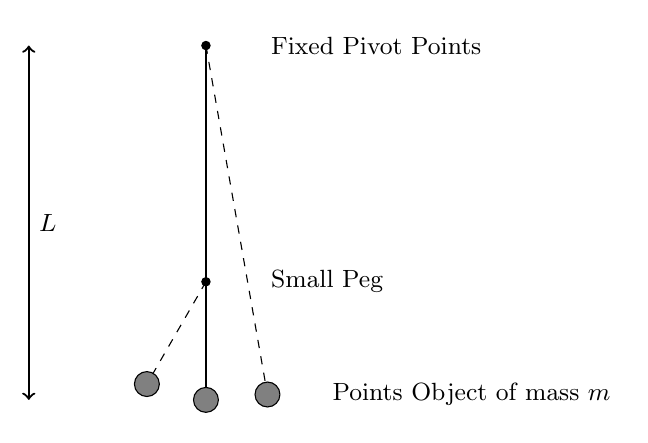
\begin{tikzpicture}[scale=1.5,font=\small]
        %% Length label
        \draw[thick,<->] (-1.5,-1) -- (-1.5,2) node[pos=0.5,anchor=west] {$L$};
        \draw (0,-1) -- (0,2);
        %% Pegs
        \draw[fill] (0,2) circle (1pt) node[anchor=west,xshift=2em] {Fixed Pivot Points};
        \draw[fill] (0,0) circle (1pt) node[anchor=west,xshift=2em] {Small Peg};
        \draw[dashed] (0,2) -- ++(280:3);
        \draw[fill=white!50!black] (0,2) ++(280:3) circle (3pt)  node[anchor=west,xshift=2em] {Points Object of mass $m$};
        \draw[dashed] (0,0) -- ++(240:1);
        \draw[fill=white!50!black] (0,0) ++(240:1) circle (3pt);
        \draw[fill=white!50!black] (0,-1) circle (3pt);
    \end{tikzpicture}
    \end{center}
    The mass is displaced 5 degrees from the vertical and released.
    How long does it take to return to its starting position?
    \begin{multicols}{2}
    \begin{choices}
        \wrongchoice{$\pi \sqrt{\dfrac{L}{g}\left(1+\sqrt{\dfrac{2}{3}}\right)}$}
        \wrongchoice{$\pi \sqrt{\dfrac{L}{g}\left(2+\dfrac{2}{\sqrt{3}}\right)}$}
        \wrongchoice{$\pi \sqrt{\dfrac{L}{g}\left(2+\dfrac{1}{3}\right)}$}
        \wrongchoice{$\pi \sqrt{\dfrac{L}{g}\left(2+\sqrt{3}\right)}$}
      \correctchoice{$\pi \sqrt{\dfrac{L}{g}\left(2+\frac{1}{\sqrt{3}}\right)}$}
    \end{choices}
    \end{multicols}
\end{question}
}

\element{aapt}{ %% Olympiad-A8
\begin{question}{Olympiad-2009-q23}
    A mass is attached to an ideal spring.
    At time $t=0$ the spring is at its natural length and the mass is given an initial velocity;
        the period of the ensuing (one-dimensional) simple harmonic motion is $T$.
    At what time is the power delivered to the mass by the spring first a maximum?
    \begin{multicols}{3}
    \begin{choices}
        \wrongchoice{$t=\text{zero}$}
        \wrongchoice{$t=\dfrac{T}{8}$}
        \wrongchoice{$t=\dfrac{T}{4}$}
      \correctchoice{$t=\dfrac{3T}{8}$}
        \wrongchoice{$t=\dfrac{T}{2}$}
    \end{choices}
    \end{multicols}
\end{question}
}


%% PhysicsOlympiad 2008
%%----------------------------------------
\element{aapt}{ %% Olympiad-A8
\begin{question}{Olympiad-2008-q13}
    A mass is attached to the wall by a spring of constant $k$.
    When the spring is at its natural length,
        the mass is given a certain initial velocity,
        resulting in oscillations of amplitude $A$.
    If the spring is replaced by a spring of constant $2k$,
        and the mass is given the same initial velocity,
        what is the amplitude of the resulting oscillation?
    \begin{multicols}{3}
    \begin{choices}
        \wrongchoice{$\dfrac{1}{2}A$}
      \correctchoice{$\dfrac{1}{\sqrt{2}}A$}
        \wrongchoice{$\sqrt{2}A$}
        \wrongchoice{$2A$}
        \wrongchoice{$4A$}
    \end{choices}
    \end{multicols}
\end{question}
}


%% PhysicsOlympiad 2007
%%----------------------------------------


%% PhysicsOlympiad 1998
%%----------------------------------------
\element{aapt}{ %% Olympiad-A8
\begin{question}{olympiad-1998-q06}
    A pendulum is attached to the ceiling of an elevator car.
    When the car is parked, the pendulum exhibits a period of \SI{1.00}{\second}.
    The car now begins to travel upward with an upward acceleration of \SI{2.3}{\meter\per\second\squared}.
    During this part of the motion,
        what will be the approximate period of the pendulum?
    \begin{multicols}{3}
    \begin{choices}
        \wrongchoice{\SI{0.80}{\second}}
      \correctchoice{\SI{0.90}{\second}}
        \wrongchoice{\SI{1.00}{\second}}
        \wrongchoice{\SI{1.10}{\second}}
        \wrongchoice{\SI{1.20}{\second}}
    \end{choices}
    \end{multicols}
\end{question}
}


\endinput


